\documentclass[10pt, handout, envcountsect]{beamer} % text size parameter 10, ratio parameter, handout (in case of need to share)

\usetheme{Madrid} % view themes and colors at https://www.overleaf.com/learn/latex/Beamer#Reference_guide
% \usecolortheme{seahorse}

% \usepackage{pgfpages} % handouts (in case of need to share)
% \pgfpagesuselayout{4 on 1}[a4paper, border shrink=5mm]

\setbeamertemplate{navigation symbols}{} % hides navigation buttons at buttom 
%\setbeamertemplate{footline}[frame number]{} % gets rid of bottom navigation bars
\setbeamercovered{transparent} % makes transparent paramters

\setbeamertemplate{headline}{} % hides navigation bar on top

\usepackage{graphicx} % Required for inserting images
\title[Paper Review]{Paper Review}
\subtitle{
\large{Data augmentation in Bayesian neural networks and the cold posterior effect}
\\
\vspace{3pt}
\normalsize{Seth Nabarro \textit{et al.}}
}
\author{Marat Khusainov}
\date{April 2024}

\begin{document}

\maketitle

% ------------------------------

\begin{frame}{Outline}

\tableofcontents

\end{frame}

\section{Motivation}
% ------------------------------


% \section{Problem Statement}
% ------------------------------
\begin{frame}{Motivation}
\textbf{The cold posterior effect}
\begin{equation}
\mathrm{P}(\mathbf{w} \mid \mathbf{y}, \mathbf{X}) \propto \mathrm{P}(\mathbf{w}) \mathrm{P}(\mathbf{y} \mid \mathbf{w}, \mathbf{X}) \tag{1}
\end{equation}
Better performance when using a “cold” posterior:
\begin{equation*}
\mathrm{Q}(\mathbf{w}) \propto(\mathrm{P}(\mathbf{w}) \mathrm{P}(\mathbf{y} \mid \mathbf{w}, \mathbf{X}))^{1 / T} \tag{2} \text{, where $T<1$.}
\end{equation*}

\begin{itemize}
    \vspace{7pt}
    \item One possible explanation is that the CPE is an artifact of data augmentation.
    \vspace{3pt}
    \item It is important to investigate integrating DA with Bayesian neural networks, and to examine the interaction with the CPE.
    % \item 


\end{itemize}
\end{frame}




\section{Methods}
% ------------------------------


\begin{frame}{Methods}
To incorporate DA into BNN likelihoods, define the probabilities for each class as being averages over augmentations.
Authors choose to either average logits (equal to the neural network outputs, $\mathbf{f}(\cdot ; \mathbf{w}))$ or predictive probabilities $(\operatorname{softmax} \mathbf{f}(\cdot ; \mathbf{w}))$,
\begin{align*}
\mathbf{p}_{\text {inv }}\left(\mathbf{x}_{i} ; \mathbf{w}\right) & =\mathbb{E}\left[\operatorname{softmax} \mathbf{f}\left(\mathbf{x}_{i}^{\prime} ; \mathbf{w}\right)\right]  \tag{3}\\
\mathbf{f}_{\text {inv }}\left(\mathbf{x}_{i} ; \mathbf{w}\right) & =\mathbb{E}\left[\mathbf{f}\left(\mathbf{x}_{i}^{\prime} ; \mathbf{w}\right)\right] . \tag{4}
\end{align*}

where expectations over $\mathrm{P}\left(\mathbf{x}_{i}^{\prime} \mid \mathbf{x}_{i}\right), \mathbf{x}_{i}^{\prime}$ -- augmented input.

\vspace{8pt}

The resulting (usually intractable) log-likelihoods are
\begin{align*}
\mathcal{L}_{\text {prob }}^{i}\left(y_{i} ; \mathbf{w}\right) & =\log \mathrm{P}_{\text {prob }}\left(y_{i} \mid \mathbf{x}_{i}, \mathbf{w}\right) \\
& =\log \mathbb{E}\left[\operatorname{softmax}_{y_{i}} \mathbf{f}\left(\mathbf{x}_{i}^{\prime} ; \mathbf{w}\right)\right]  \tag{5}\\
\mathcal{L}_{\text {logits }}^{i}\left(y_{i} ; \mathbf{w}\right) & =\log \mathrm{P}_{\text {logits }}\left(y_{i} \mid \mathbf{x}_{i}, \mathbf{w}\right) \\
& =\log \operatorname{softmax}_{y_{i}} \mathbb{E}\left[\mathbf{f}\left(\mathbf{x}_{i}^{\prime} ; \mathbf{w}\right)\right] \tag{6}
\end{align*}





\end{frame}

\begin{frame}{Methods}
Authors show that it is possible to get tight, intuitive and easy to evaluate, multi-sample bounds analogous to those in IWAE \footnote{\href {https://arxiv.org/pdf/1509.00519.pdf}{Burda
et al., 2015, Importance weighted autoencoders.}}.
\begin{align*}
& \hat{\mathcal{L}}_{\text {prob }, K}^{i}\left(y_{i} ; \mathbf{w}\right)=\log \left(\frac{1}{K} \sum_{k=1}^{K} \operatorname{softmax}_{y_{i}} \mathbf{f}\left(\mathbf{x}_{i ; k}^{\prime} ; \mathbf{w}\right)\right), \\
& \hat{\mathcal{L}}_{\text {logits }, K}^{i}\left(y_{i} ; \mathbf{w}\right)=\log \operatorname{softmax}_{y_{i}}\left(\frac{1}{K} \sum_{k=1}^{K} \mathbf{f}\left(\mathbf{x}_{i ; k}^{\prime} ; \mathbf{w}\right)\right) . \tag{7}
\end{align*}

Increasing $K$ reduces the variance and tightens the bounds which eventually become exact as $K \rightarrow \infty$ .

\begin{align*}
\mathcal{L}_{\text {logits }}^{i}\left(y_{i} ; \mathbf{w}\right) & =\lim _{K \rightarrow \infty} \hat{\mathcal{L}}_{\text {logits }, K}^{i}\left(y_{i} ; \mathbf{w}\right)  \tag{8}\\
\mathcal{L}_{\text {prob }}^{i}\left(y_{i} ; \mathbf{w}\right) & =\lim _{K \rightarrow \infty} \hat{\mathcal{L}}_{\text {prob }, K}^{i}\left(y_{i} ; \mathbf{w}\right) \tag{9}
\end{align*}
\end{frame}

\end{frame}



\begin{frame}{Methods}
The authors propose two types of settings.

\vspace{10pt}

\begin{itemize}
\item The usual \textbf{“full orbit”} setting,
where there is a distribution over a very large, or even infinite number of possible augmentations.
The full orbit setting
necessitates the use of the bound (Eq.7).

\vspace{10pt}

\item Alternative \textbf{“finite orbit”} by restricting the augmentations to
a small subset, we can exactly evaluate the log-likelihood. In the finite orbit setting, the distribution over augmented
images, $\mathbf{x}_{i}^{\prime}$
, conditioned on the underlying unaugmented image, $\mathbf{x}_{i}$
, can be written as

\begin{equation*}
\mathrm{P}\left(\mathbf{x}_{i}^{\prime} \mid \mathbf{x}_{i}\right)=\frac{1}{K} \sum_{k=1}^{K} \delta\left(\mathbf{x}_{i}^{\prime}-a_{k}\left(\mathbf{x}_{i}\right)\right), \tag{10}
\end{equation*}
and $a_{k}$ is a function that applies the $k$ th fixed augmentation.
\end{itemize}
\end{frame}

\begin{frame}{Results }
\begin{figure}[h]
    \centering
    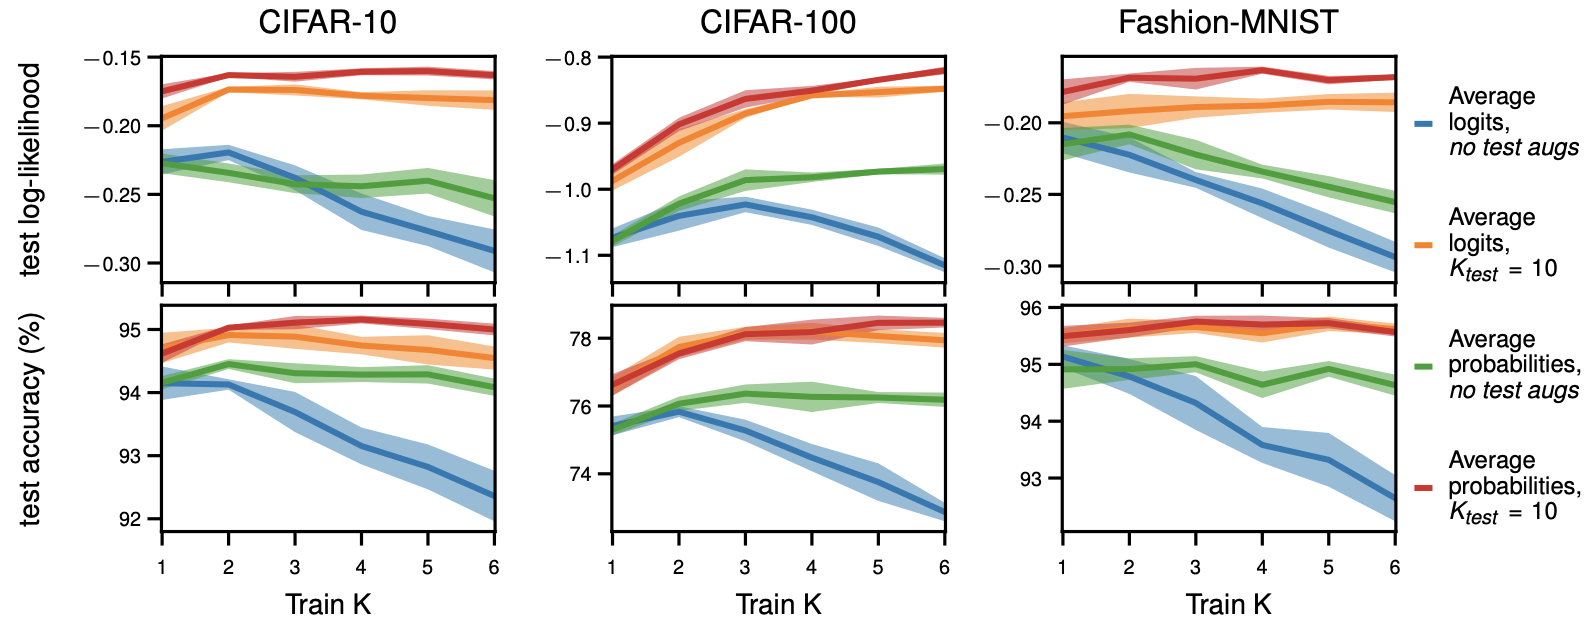
\includegraphics[width=11cm,]{figure2.png}
    \caption{Comparison of averaging logits and probabilities for different values of $K_{\text {train }}$, and using $K_{\text {test }}=10$ vs. using no test-time augmentations. Here, we use ResNet18 with SGD (i.e. no Bayesian inference). We use only full orbit to decouple $K_{\text {train }}$ from $K_{\text {test }}$.}
    % \label{}
\end{figure}
\end{frame}

\begin{frame}{Results}

\begin{figure}[h]
    \centering
    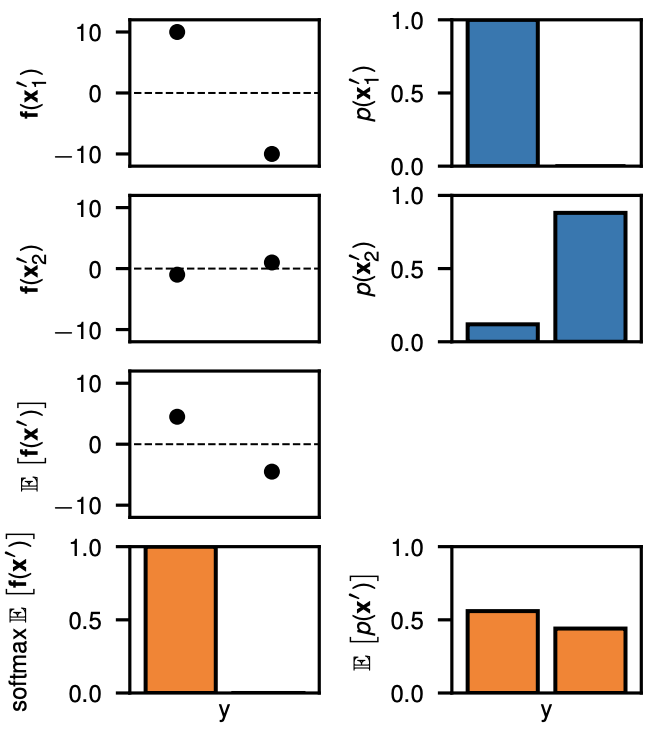
\includegraphics[width=6cm,]{figure3.png}
    \caption{Example effect of averaging logits against averaging probabilities. 
    }
    % \label{}
\end{figure}


    
\end{frame}





% ------------------------------
\section{Experiment}
% ------------------------------
\begin{frame}{Results}

\begin{figure}[h]
    \centering
    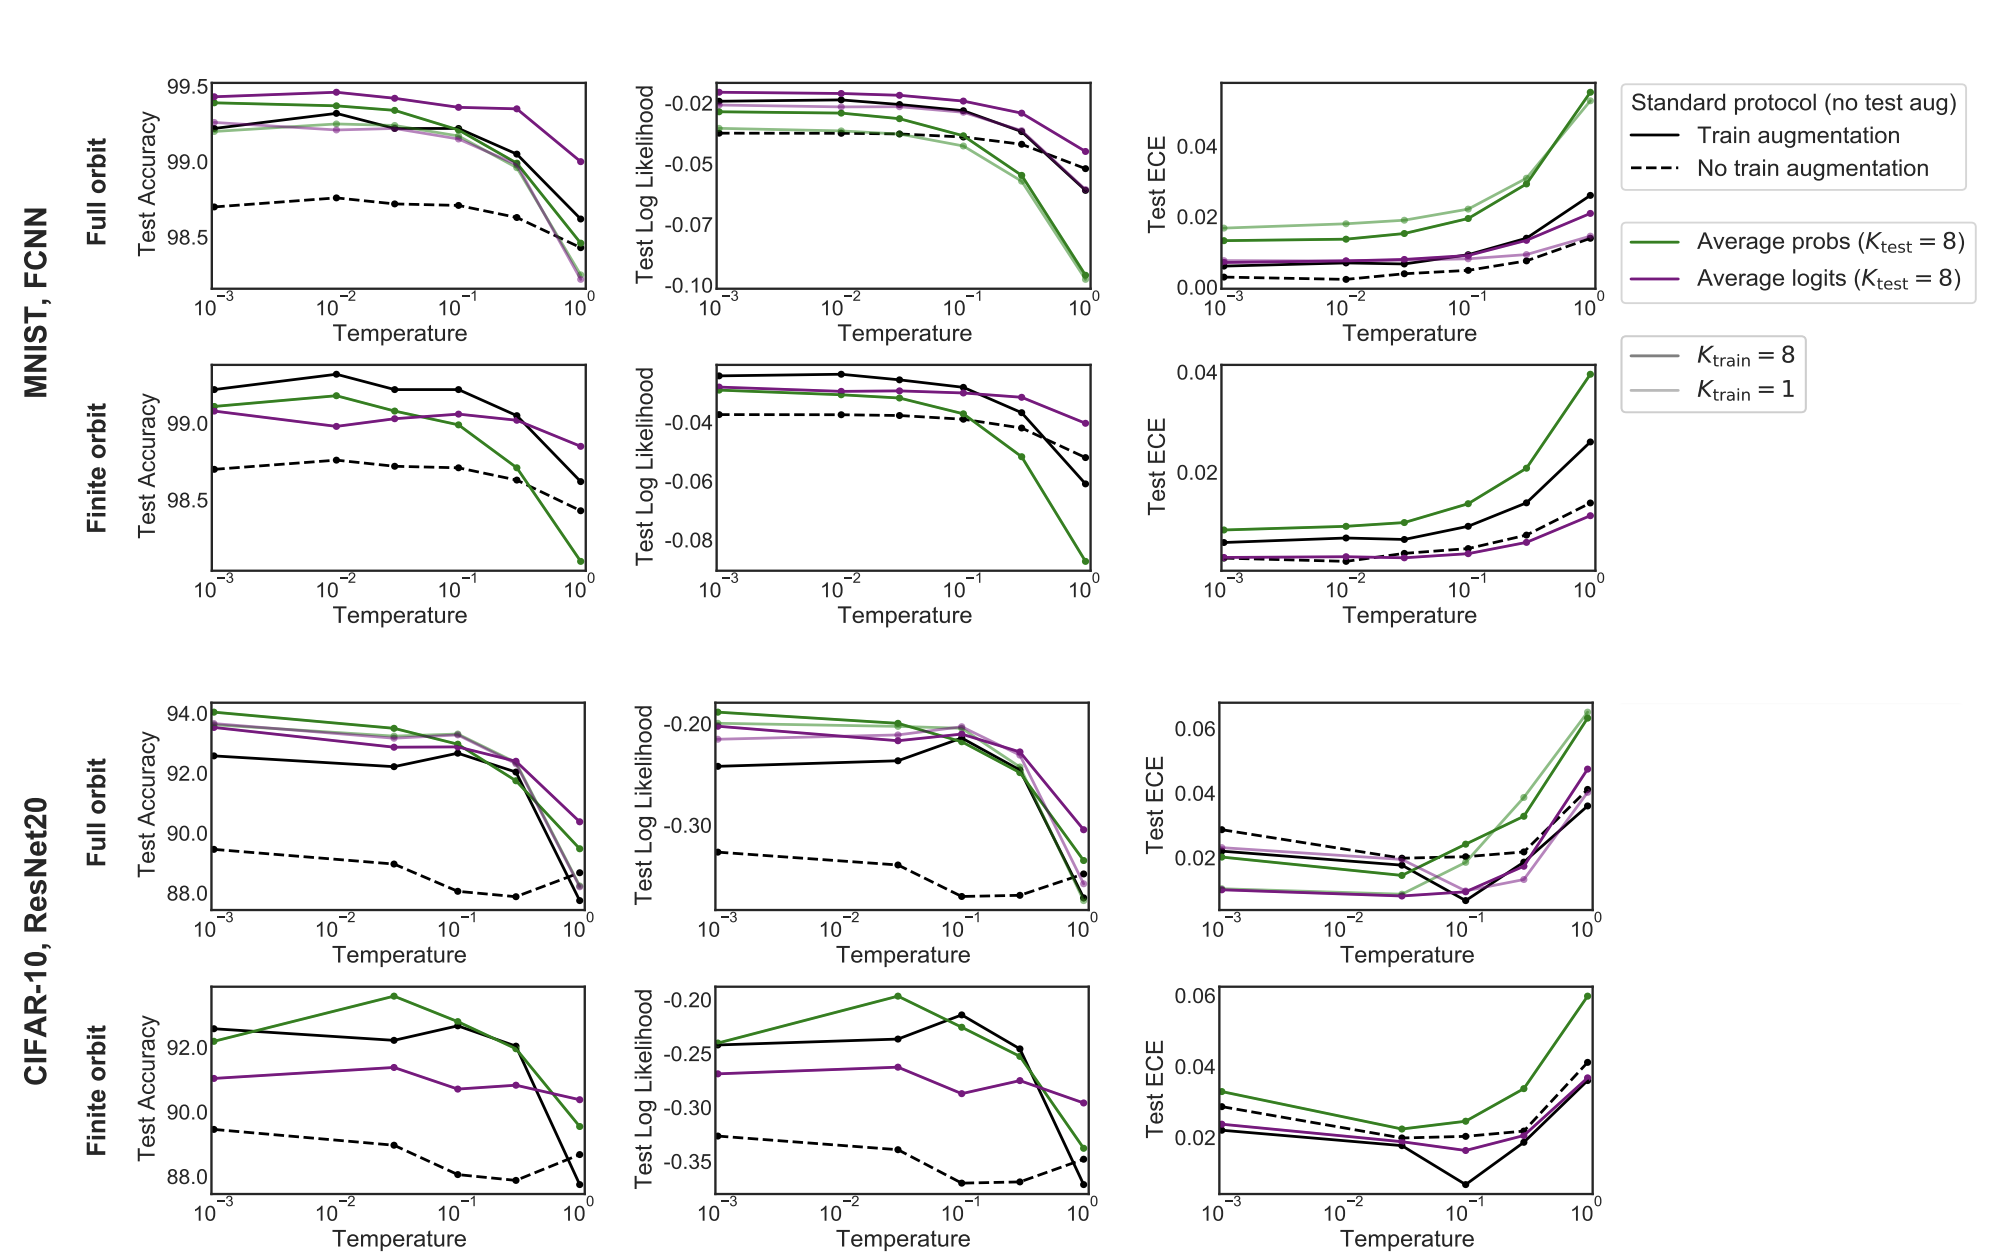
\includegraphics[width=11cm,]{figure4.png}
    \caption{The cold posterior effect for different DA setups.}
    % \label{}
\end{figure}


    
\end{frame}





\section{Conclusion}

\begin{frame}{Conclusion}
\begin{itemize}
    \item  Shown how DA can be properly incorporated into
a model suitable for BNN inference, by deriving
a lower-bound on the log-likelihood of the augmentation averaged network output.

\vspace{10pt}

    \item Empirically, seen that the
CPE persists even when using our principled DA formulation, shown that the CPE disappears without DA.
\end{itemize}
\end{frame}
\end{document}

